\documentclass[12pt,a4paper]{report}
\usepackage[utf8]{inputenc}
\usepackage[T1]{fontenc}
\usepackage{lmodern}
\usepackage{amsmath,amssymb}
\usepackage{graphicx}
\usepackage{booktabs,longtable,array,calc}
\usepackage{microtype}
\usepackage[a4paper,top=2cm,bottom=2cm,left=2.5cm,right=2.5cm]{geometry}
\usepackage{tikz}
\usetikzlibrary{arrows.meta}
\usepackage{xcolor}
\usepackage[hidelinks]{hyperref}
\usepackage{parskip}
\usepackage{textcomp}
\usepackage{newunicodechar}
\newunicodechar{§}{\S}
\newunicodechar{·}{\textperiodcentered}
\newunicodechar{…}{\ldots}
\newunicodechar{–}{--}
\newunicodechar{—}{---}
\newunicodechar{°}{\textdegree}
\newunicodechar{±}{\ensuremath{\pm}}
\newunicodechar{×}{\ensuremath{\times}}
\newunicodechar{≈}{\ensuremath{\approx}}
\newunicodechar{≠}{\ensuremath{\neq}}
\newunicodechar{≥}{\ensuremath{\geq}}
\newunicodechar{≤}{\ensuremath{\leq}}
\newunicodechar{→}{\ensuremath{\rightarrow}}
\newunicodechar{←}{\ensuremath{\leftarrow}}
\newunicodechar{−}{\ensuremath{-}}
\newunicodechar{∇}{\ensuremath{\nabla}}
\newunicodechar{∅}{\ensuremath{\emptyset}}
\newunicodechar{△}{\ensuremath{\triangle}}
\newunicodechar{θ}{\ensuremath{\theta}}
\newunicodechar{π}{\ensuremath{\pi}}
\newunicodechar{α}{\ensuremath{\alpha}}
\newunicodechar{†}{\textdagger}
\newunicodechar{⚠}{\textbf{!}}

% --- pandoc helper macros (fragment mode needs these) ---
\providecommand{\tightlist}{\setlength{\itemsep}{0pt}\setlength{\parskip}{0pt}}
\providecommand{\passthrough}[1]{#1}
\providecommand{\pandocbounded}[1]{#1}
\providecommand{\real}[1]{#1}

\usepackage{listings}
\lstset{basicstyle=\ttfamily\footnotesize,breaklines=true,breakatwhitespace=false,
  columns=fullflexible,keepspaces=true,showstringspaces=false,frame=none,
  breakindent=0pt,postbreak=\mbox{\textcolor{gray}{$\hookrightarrow$}\space}}
\usepackage{etoolbox}
\AtBeginEnvironment{longtable}{\small}
\AtBeginEnvironment{verbatim}{\footnotesize}

\setcounter{secnumdepth}{3}
\setcounter{tocdepth}{2}

% compact chapter headings (less blank space at the top of chapter/appendix pages)
\usepackage{titlesec}
\titleformat{\chapter}[display]{\normalfont\bfseries\Huge}{\chaptertitlename\ \thechapter}{6pt}{\Huge}
\titlespacing*{\chapter}{0pt}{4pt}{16pt}

\begin{document}

% ============================ TITLE PAGE ============================
\begin{titlepage}
\centering
{\large [VNUHCM] University of Science\par}     % TODO: confirm
{\large Faculty of [Information Technology]\par} % TODO: GVHD/khoa
\vspace{1.5cm}
{\large Bachelor's Thesis\par}
\vspace{2cm}
{\Large\bfseries Accelerating Test-Time Discovery in Complex Code Generation via Execution-Guided Self-Distillation\par}
\vspace{1cm}
{\color{red}\small\itshape Draft for format/framing review --- contains placeholder data ($\S$4.2.5); see \texttt{PLACEHOLDERS.md}.\par}
\vspace{1.5cm}
\begin{flushright}\large
\textbf{Student:} Mai Dang \quad (MSSV: \underline{\hspace{2.5cm}})\\[0.5em]
\textbf{Supervisor:} \underline{\hspace{5cm}}\\[0.5em]   % TODO: GVHD
\end{flushright}
\vfill
{\large Ho Chi Minh City, 2026\par}              % TODO: confirm year
\end{titlepage}

\chapter*{Abstract}
\addcontentsline{toc}{chapter}{Abstract}
\input{_abstract.tex}

\tableofcontents

\chapter{Chapter 1 --- Introduction}\label{chapter-1-introduction}

This thesis studies how to \textbf{accelerate test-time discovery in complex code generation via execution-guided self-distillation}. The core question is practical: when a language model is given a single hard programming problem and a budget to improve itself at inference time, what is the most effective way to turn execution feedback into a better solution, and when does that strategy work?

\section{1.1 Background}\label{background}

Reinforcement learning with verifiable rewards (RLVR) is the standard recipe for post-training language models on code and math, with GRPO {[}8{]} as a common instantiation. Its weakness is sparse credit assignment: a scalar outcome reward says only whether an attempt passed, not where it went wrong, and when every sampled rollout fails, the advantage collapses and learning stalls. This failure is most acute on exactly the problems that matter, the hard ones, where successes are rare.

Self-Distillation Policy Optimization (SDPO) {[}1{]} addresses this by extracting a denser signal from the \emph{rich feedback} that verifiable environments already produce but usually discard, such as runtime errors and failing tests. The same model, conditioned on this feedback, acts as a self-teacher whose retrospective per-token distribution is distilled back into the student. At test time, SDPO can iterate on a single hard problem and improve before it ever produces a first success, measured by discovery@k, the probability of solving within the first \(k\) attempts {[}1, §5{]}.

Two open issues motivate this work. First, the parent paper organizes its update \emph{student-first}: it distills the student's own failed rollout. On a problem the bare student rarely solves, those rollouts are almost never correct, so there is little that is right to learn from. Second, Kim et al.~{[}2{]} show that distilling from rich context can degrade a model by suppressing its epistemic verbalization, which raises the question of whether the feedback helps the model reason or merely teaches it to copy.

\section{1.2 Problem}\label{problem}

The setting is test-time training (TTT): one hard problem, a verifiable reward, and a short budget of self-improvement steps, after which the model is reset. Two design choices govern how well the model discovers a solution. One is \emph{how the execution feedback is organized into a learning signal}: should the model learn from its own failed attempt, or from a correct attempt produced under feedback and filtered for independence? The other is \emph{how the execution feedback is formulated} into the reprompt the self-teacher sees, which the parent paper leaves as an explicit open question {[}1, §7{]}. This thesis takes execution feedback as the privileged context that guides self-distillation, hence \emph{execution-guided}, and studies both choices with the goal of accelerating discovery.

\section{1.3 Research questions}\label{research-questions}

Two primary questions drive the study:

\begin{itemize}
\tightlist
\item
  \textbf{RQ-method.} At test time, does a teacher-first organization, which distills filtered teacher-generated trajectories, beat the student-first baseline, which distills the student's own failed rollout, at discovering solutions to hard code problems?
\item
  \textbf{RQ1.} Does the reprompt-template formulation of the execution feedback affect discovery, and in which regime?
\end{itemize}

Two secondary, exploratory questions situate the work within the wider self-distillation literature:

\begin{itemize}
\tightlist
\item
  \textbf{RQ2 (exploratory).} Does self-distillation from rich context suppress epistemic verbalization at test time? Only a limited math pilot bears on this, since the code runs produce no reasoning trace.
\item
  \textbf{RQ3 (exploratory).} How does discovery trade off against compute? This thesis quantifies the compute overhead of teacher-first and identifies the compute-matched comparison a full answer requires; the compute-to-correct Pareto itself is left to future work (§4.2.5, §6.2.4).
\end{itemize}

\section{1.4 Contributions}\label{contributions}

The contributions are stated at the strength the evidence supports; the sample sizes are small and the claims are directional, never proofs.

\begin{enumerate}
\def\labelenumi{\arabic{enumi}.}
\tightlist
\item
  \textbf{A teacher-first variant of execution-guided self-distillation.} A method that distills the student toward verifier- and judge-filtered trajectories generated by the self-teacher, positioned between on-policy SDPO and off-policy SFT (Chapter 3).
\item
  \textbf{Evidence that teacher-first accelerates discovery where on-policy SDPO stalls.} Across matched comparisons, teacher-first is at least as good as student-first on every seed and never worse, and on the hardest problems it escapes the flat-reward trap that keeps student-first stuck at zero. This escape-zero behavior is replicated three times, with one case improving the pass-rate roughly ninefold (Chapter 4).
\item
  \textbf{A reprompt-template effect.} The formulation of the execution feedback affects discovery, most clearly on hard problems, where a reasoning-inducing template orders above the plain anchor, which orders above a minimal one (§4.3).
\item
  \textbf{A value-versus-procedure boundary characterization.} A math pilot shows where the method does \emph{not} help: when the reference encodes only an answer rather than an in-reach method, the teacher copies the answer (a copy rate near 75\% is measured), the leak transfers reasoning style but not capability, and the student stays at zero. This characterizes escape as requiring reachable capability and a method-bearing reference, not merely a correct answer (§4.5, Chapter 5).
\end{enumerate}

\section{1.5 Scope}\label{scope}

The study is confined to the test-time training regime: single-problem self-improvement with a per-problem reset, using LoRA adapters, which is the appropriate lightweight choice for adapting to one problem at inference time. Code generation on LiveCodeBench v6 {[}6{]} is the core, carrying the main claims; an AIME 2026 math pilot serves as a contrast that characterizes the boundary of the mechanism. Results are on one 4B-scale model per domain, an anchor template for the main comparison, and a 15-step budget. No claim of universality is made.

\section{1.6 Thesis structure}\label{thesis-structure}

Chapter 2 reviews the background and related work: RLVR and GRPO, SDPO and its loss, test-time training and discovery@k, the reprompt-template design space, and the epistemic-suppression literature. Chapter 3 specifies the method, including the student-first baseline, the proposed teacher-first organization, the template taxonomy, the two domains, and the metrics. Chapter 4 reports the experiments: the main teacher-first versus student-first comparison and the escape-zero result, the template study, the robustness ablations, and the math pilot. Chapter 5 discusses the mechanism and the value-versus-procedure boundary. Chapter 6 states the limitations and the future experiments that would address them. Chapter 7 concludes.

\section{In-chapter citations}\label{in-chapter-citations}

Numbered per the master bibliography (\texttt{00\_references.md}): {[}1{]} Hübotter et al.~2026 · {[}2{]} Kim et al.~2026 · {[}6{]} LiveCodeBench · {[}8{]} GRPO / DeepSeekMath.

\input{_ch2.tex}
\input{_ch3.tex}
\chapter{Chapter 4 --- Experiments}\label{chapter-4-experiments}

This chapter reports the empirical results. The structure follows the framing of Chapter 3: code is the core and carries the main claims, math is a pilot that characterizes the boundary of the mechanism.

The experiments answer three questions. First, the method question (RQ-method): does the proposed teacher-first organization beat the student-first baseline at test-time discovery, and if so where and how much (§4.2)? Second, RQ1: does the reprompt template matter, and in which regime (§4.3)? Third, two robustness checks: is the result invariant to the judge choice, and does the leak ablation behave as predicted (§4.4)? Section 4.5 then reports the math pilot, which does not escape and is presented as a boundary characterization rather than a failed attempt.

A standing caveat applies to every number below. The sample sizes are small (2--3 problems for the code escape results, 2 seeds for RQ1, 2 problems for math). All significance values are \textbf{crude sign tests} of the form \(0.5^k\) over non-tied matched pairs, reported as descriptive and directional evidence, never as inferential proof. The language throughout stays at ``weak / directional dominance''; nowhere is a claim stated as ``proven.''

\begin{center}\rule{0.5\linewidth}{0.5pt}\end{center}

\section{4.1 Experimental setup}\label{experimental-setup}

\textbf{Models.} Code uses Qwen3-4B {[}7{]} with LoRA (r=32, bf16), thinking OFF. Math uses Gemma-4-E4B with LoRA on all linear layers, thinking ON. The model differs across domains, which is a confound carried explicitly into every math claim (§4.5, Chapter 6).

\textbf{Hardware.} Code runs on Colab L4 (22 GB) and A100; math runs on Modal A100-80GB (Colab compute units were exhausted).

\textbf{TTT protocol.} Per problem, the model is reset to base, then run for \(K\) steps; the student is evaluated PRE and POST with no context (§3.6). Code: \(K=15\), eval 16 samples, \texttt{teacher\_n=10}. Math: \(K=3\), eval 4 samples, \texttt{teacher\_n=4}, \texttt{max\_new\_tokens=16384}. The distillation core is identical to §3.3.5 (AdamW lr=1e-5, top-K=20, \(\alpha=1.0\) reverse KL, IS clip 2.0). Full hyperparameters are in Appendix A.

\textbf{Seeds and matching.} Code uses 4 seeds (0--3). Both arms share base and seed, so PRE matches per seed, giving a paired (matched) comparison (§3.6).

\textbf{Problem selection.} Problems are chosen by \emph{model} pass-rate \(\in (0,1)\) (a model-defined frontier), not by the contest difficulty label, because a problem the model already solves or never solves carries no learning signal. The anchor template is T2 unless stated otherwise.

\begin{center}\rule{0.5\linewidth}{0.5pt}\end{center}

\section{4.2 RQ-method: teacher-first vs student-first (code)}\label{rq-method-teacher-first-vs-student-first-code}

\subsection{4.2.1 Frontier scan and the comparison design}\label{frontier-scan-and-the-comparison-design}

A frontier scan over LCBv6 problems (idx0--90) by model pass-rate identifies problems in the learnable band. Two are used for the main matched comparison: idx39 (abc393\_d, labeled hard, base pass ≈ 0.1) and idx12 (abc389\_b, labeled easy but with model pass ≈ 0.12, so \emph{model}-hard). Both arms run 4 seeds at eval-16 with PRE matched per seed.

\subsection{4.2.2 Main matched result}\label{main-matched-result}

On idx39, teacher-first (TF) is at least as good as student-first (SF) on every seed and strictly better on two:

\begin{longtable}[]{@{}lllll@{}}
\toprule\noalign{}
seed & PRE & TF POST & SF POST & TF − SF \\
\midrule\noalign{}
\endhead
\bottomrule\noalign{}
\endlastfoot
0 & 0.000 & \textbf{0.438} & 0.188 & +0.250 \\
1 & 0.000 & 0.062 & 0.000 & +0.062 \\
2 & 0.062 & 0.125 & 0.125 & 0 \\
3 & 0.188 & 0.062 & 0.062 & 0 \\
\textbf{mean} & & \textbf{0.172} & \textbf{0.094} & \textbf{+0.078} \\
\end{longtable}

On idx12, TF reaches 1.0 on all four seeds while SF wavers:

\begin{longtable}[]{@{}lllll@{}}
\toprule\noalign{}
seed & PRE & TF POST & SF POST & TF − SF \\
\midrule\noalign{}
\endhead
\bottomrule\noalign{}
\endlastfoot
0 & 0.000 & 1.000 & 0.938 & +0.062 \\
1 & 0.062 & \textbf{1.000} & 0.500 & +0.500 \\
2 & 0.062 & 1.000 & 1.000 & 0 \\
3 & 0.125 & 1.000 & 0.938 & +0.062 \\
\textbf{mean} & & \textbf{1.000} & \textbf{0.844} & +0.156 \\
\end{longtable}

Aggregating the two problems gives 8 matched seed-comparisons:

\begin{longtable}[]{@{}lllll@{}}
\toprule\noalign{}
& TF ≥ SF & TF \textgreater{} SF & tie & TF \textless{} SF \\
\midrule\noalign{}
\endhead
\bottomrule\noalign{}
\endlastfoot
idx39 (hard) & 4/4 & 2 & 2 & 0 \\
idx12 (model-hard) & 4/4 & 3 & 1 & 0 \\
\textbf{total} & \textbf{8/8} & \textbf{5} & \textbf{3} & \textbf{0} \\
\end{longtable}

Teacher-first is \textbf{≥ student-first on all 8 seeds, strictly better on 5, never worse}, and lower-variance (TF hits 1.0 on every seed of idx12 while SF ranges 0.5--1.0). The crude sign test over the 5 non-tied pairs is \(0.5^5 \approx 0.03\). The pattern repeats across two independent problems, which argues against pure sampling noise. The honest reading is \textbf{weak dominance}: many ties, modest typical margins, and the large wins are seed-specific.

A control observation supports that the effect is real rather than an artifact of TF being more aggressive. On idx39 seed 3, where PRE is already high (0.188), \emph{both} arms degrade identically. This is over-distillation when the base starts strong, and it applies to both arms equally, so it is not a TF-specific failure.

The aggregate means are shown in Figure 4.1 and the per-seed trajectories in Figure 4.2.

\begin{center}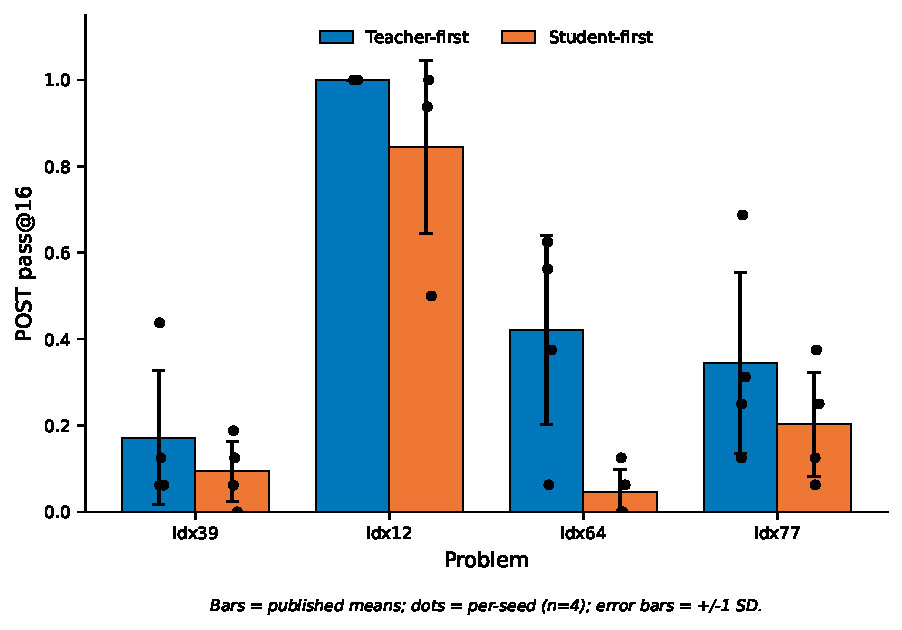
\includegraphics[width=0.85\linewidth]{../figures/fig_4_1_main_result.pdf}\end{center}

\textbf{Figure 4.1}
\emph{POST pass@16, teacher-first versus student-first.} Bars are the published means; dots are per-seed values (\(n=4\), all four problems, recovered and verified from the W\&B export); error bars are \(\pm 1\) SD. Teacher-first is at or above student-first on every problem.

\begin{center}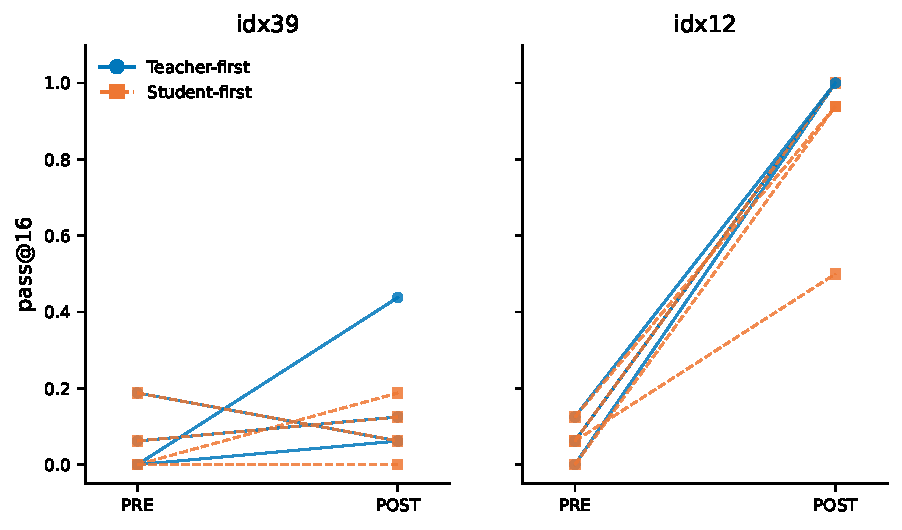
\includegraphics[width=0.85\linewidth]{../figures/fig_4_2_per_seed_slope.pdf}\end{center}

\textbf{Figure 4.2}
\emph{Per-seed PRE→POST change.} Each line is one seed. Teacher-first (solid) is at or above student-first (dashed) on every seed; teacher-first reaches 1.0 on all seeds of idx12 while student-first varies.

\subsection{4.2.3 Hard-frontier escape-zero}\label{hard-frontier-escape-zero}

The main result is weak dominance. The sharper claim comes from extending the matched comparison to harder, lower-pass problems, to test the flat-reward-trap hypothesis directly: on-policy SF should stay stuck at zero where the bare student rarely rolls a correct attempt, while TF escapes because the teacher can generate a correct solution to distill.

\begin{longtable}[]{@{}
  >{\raggedright\arraybackslash}p{(\columnwidth - 12\tabcolsep) * \real{0.1429}}
  >{\raggedright\arraybackslash}p{(\columnwidth - 12\tabcolsep) * \real{0.1429}}
  >{\raggedright\arraybackslash}p{(\columnwidth - 12\tabcolsep) * \real{0.1429}}
  >{\raggedright\arraybackslash}p{(\columnwidth - 12\tabcolsep) * \real{0.1429}}
  >{\raggedright\arraybackslash}p{(\columnwidth - 12\tabcolsep) * \real{0.1429}}
  >{\raggedright\arraybackslash}p{(\columnwidth - 12\tabcolsep) * \real{0.1429}}
  >{\raggedright\arraybackslash}p{(\columnwidth - 12\tabcolsep) * \real{0.1429}}@{}}
\toprule\noalign{}
\begin{minipage}[b]{\linewidth}\raggedright
problem
\end{minipage} & \begin{minipage}[b]{\linewidth}\raggedright
id
\end{minipage} & \begin{minipage}[b]{\linewidth}\raggedright
judge
\end{minipage} & \begin{minipage}[b]{\linewidth}\raggedright
SF mean
\end{minipage} & \begin{minipage}[b]{\linewidth}\raggedright
TF mean
\end{minipage} & \begin{minipage}[b]{\linewidth}\raggedright
win/tie/loss
\end{minipage} & \begin{minipage}[b]{\linewidth}\raggedright
escape-zero
\end{minipage} \\
\midrule\noalign{}
\endhead
\bottomrule\noalign{}
\endlastfoot
idx39 & abc393\_d & difflib & 0.094 & 0.172 & 2/2/0 & seed1 (SF 0→0, TF 0.062) \\
idx64 & abc397\_e & LLM-groq & 0.047 & \textbf{0.422} & 4/0/0 & seed1 (SF 0.062→0, TF 0.375), seed2 (SF 0→0, TF 0.062) \\
idx77 & abc399\_f & difflib & 0.203 & 0.344 & 3/1/0 & --- (SF not stuck at 0 here) \\
\textbf{total} & & & & & \textbf{9/3/0} & \textbf{3 instances / 2 problems} \\
\end{longtable}

Three findings. TF beats SF on all three hard problems and never loses; the crude sign test over the 9 non-tied pairs is \(0.5^9 \approx 0.002\). \textbf{Escape-zero replicates three times} (idx39 s1, idx64 s1 and s2): SF stays at or falls back to pass = 0 while TF escapes. This is the direct mechanistic signature predicted in §3.6: the on-policy flat-reward trap versus off-policy injection. idx64 is the strongest case, TF 0.422 versus SF 0.047 (roughly 9×), winning 4/4.

Two honest caveats. idx39 appears in both §4.2.2 and this table, so the two groupings are not independent. And the judge differs across problems (idx64 uses the LLM judge, idx39/77 use difflib), which is acceptable only because §4.4 separately establishes judge-invariance.

\begin{center}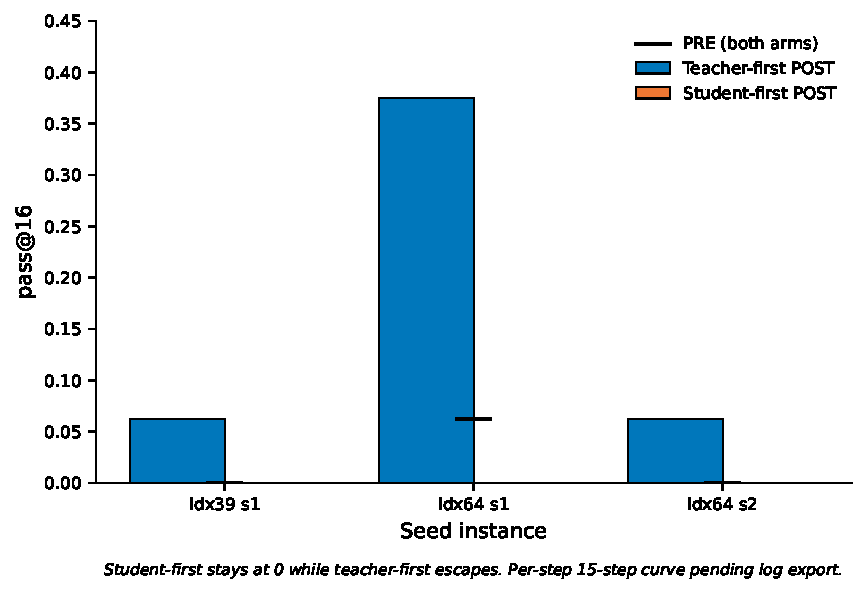
\includegraphics[width=0.85\linewidth]{../figures/fig_4_3_escape_zero.pdf}\end{center}

\textbf{Figure 4.3}
\emph{Escape-zero instances.} On three seeds, student-first POST stays at 0 (or falls back to it) while teacher-first lifts off zero. Black marks are PRE (shared by both arms). The per-step 15-step discovery curve is pending log export.

\begin{quote}
\textbf{Claim, calibrated.} The contribution is not ``TF wins by a small margin.'' It is: \emph{teacher-first learns on hard problems where on-policy SDPO is caught in a flat-reward trap, the margin is large, and escape-zero is replicated.} The claim is bounded by n: 2--3 problems, one 4B model, template T2, and no compute matching (TF generates roughly 2.5× more, so it wins on outcome, not yet on compute).
\end{quote}

\subsection{4.2.4 Discovery curves and qualitative behavior}\label{discovery-curves-and-qualitative-behavior}

Beyond aggregate pass-rate, the runs show genuine discovery rather than confidence inflation. On idx12, greedy decoding moves 0.075 → 1.0; on idx39, 0.175 → 0.225. The model learns to solve problems it deterministically failed before. One concrete trace (full excerpt in Appendix D.5): idx12 base uses \texttt{math.factorial(X)} in the wrong direction, the feedback reports a runtime error, and the model learns to iterate to find N. In an exploratory run (idx29), the base calls \texttt{exit()} (unavailable in the sandbox), the feedback reports a \texttt{NameError}, and the model corrects it.

Two further observations. On easy-to-fix exploratory problems (idx23, idx29 at eval-8), both arms solve almost equally, so differentiation is clearer on harder problems. And from around step 2 the teacher tends to converge (batch reward = 1.0, mean similarity ≈ 0.9, \texttt{n\_good} → 1); when the base starts high, both arms can over-distill, consistent with the idx39 seed-3 control above.

\subsection{4.2.5 Compute considerations (RQ3, partial)}\label{compute-considerations-rq3-partial}

The comparisons above are matched on seeds and on the step budget, but not on generations. Teacher-first draws \texttt{teacher\_n=10} samples per step against student-first's four, roughly a 2.5× generation overhead, so the results establish an outcome advantage rather than a compute-fair one. Two observations bound what can be said. The discovery curves (§4.2.4) show teacher-first reaching a high pass-rate within the 15-step budget, and the escape-zero seeds show student-first failing across its own 60 generations (4 per step over 15 steps) while teacher-first escapes. This points to the \emph{kind} of distilled trajectory, rather than raw sample volume, as the driver of the gap.

The point is suggestive, not conclusive. Student-first was never run at teacher-first's generation budget, and no best-of-k baseline was measured at matched compute, so more student-first sampling cannot be ruled out as an alternative route to escape. A full answer needs a compute-to-correct frontier that holds total generations fixed and logs token and GPU-time cost; §6.2.4 sets this out as future work. RQ3 is therefore answered only in part here: the overhead is quantified and the missing comparison is identified, but the Pareto trade-off itself is not measured.

\begin{center}\rule{0.5\linewidth}{0.5pt}\end{center}

\section{4.3 RQ1: the reprompt template}\label{rq1-the-reprompt-template}

RQ1 probes the titular question directly. Holding the SF arm fixed (script 07, Qwen3-4B, thinking OFF, 15 steps, eval-16), three templates were run on two problems at 2 seeds each. POST pass@16:

\begin{longtable}[]{@{}
  >{\raggedright\arraybackslash}p{(\columnwidth - 4\tabcolsep) * \real{0.3333}}
  >{\raggedright\arraybackslash}p{(\columnwidth - 4\tabcolsep) * \real{0.3333}}
  >{\raggedright\arraybackslash}p{(\columnwidth - 4\tabcolsep) * \real{0.3333}}@{}}
\toprule\noalign{}
\begin{minipage}[b]{\linewidth}\raggedright
Template
\end{minipage} & \begin{minipage}[b]{\linewidth}\raggedright
idx12 (easy)
\end{minipage} & \begin{minipage}[b]{\linewidth}\raggedright
idx39 (hard)
\end{minipage} \\
\midrule\noalign{}
\endhead
\bottomrule\noalign{}
\endlastfoot
T1\_minimal (``provide a corrected solution'') & 0.66 & \textbf{0.03} \\
T2\_standard (``correctly solve the original question'') & 0.97 & 0.06 \\
T5\_reasoning (``identify root cause, then provide corrected'') & 0.97 & \textbf{0.13} \\
\end{longtable}

On the hard problem the ordering is monotone, \textbf{T5 \textgreater{} T2 \textgreater{} T1} (0.13 \textgreater{} 0.06 \textgreater{} 0.03), and T5 is stable across its two seeds (.125 / .125). A reasoning-inducing reprompt beats the plain anchor, which beats the minimal one. On the easy problem T2 and T5 saturate together near 0.97 while T1 drops to 0.66 (partly one unlucky seed).

The template has an effect, and that effect is clearest on the hard problem where there is room to differentiate. This is directional evidence for RQ1, not a strong-power result: n = 2 seeds and the absolute counts are small. The probe is also on the SF arm only; the template × teacher-first interaction is left for future work (Chapter 6).

\begin{center}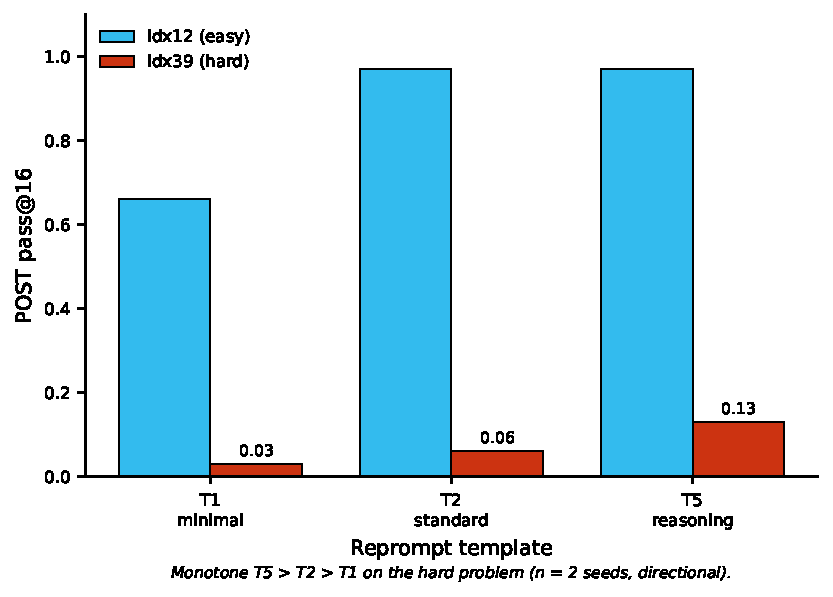
\includegraphics[width=0.85\linewidth]{../figures/fig_4_4_template.pdf}\end{center}

\textbf{Figure 4.4}
\emph{Reprompt-template effect on POST pass@16.} On the hard problem (idx39) the ordering is monotone T5 \textgreater{} T2 \textgreater{} T1; on the easy problem (idx12) T2 and T5 saturate. Directional only (\(n=2\) seeds).

\begin{center}\rule{0.5\linewidth}{0.5pt}\end{center}

\section{4.4 Robustness ablations}\label{robustness-ablations}

\subsection{4.4.1 Judge-invariance}\label{judge-invariance}

The independence judge can be a cheap string-similarity check (difflib) or a semantic LLM judge (groq \texttt{llama-3.3-70b}). Mean POST pass over 4 seeds, good\_only:

\begin{longtable}[]{@{}llll@{}}
\toprule\noalign{}
problem & SF & TF · difflib & TF · LLM \\
\midrule\noalign{}
\endhead
\bottomrule\noalign{}
\endlastfoot
idx39 & 0.094 & 0.172 & 0.266 \\
idx12 & 0.844 & 1.000 & 0.984 \\
\end{longtable}

TF ≥ SF under both judges on both problems, and the two judges give similar student POST, so the core result is \textbf{invariant to the judge choice}. The two judges do label differently: the semantic LLM calls fewer trajectories ``copy'' than difflib (on idx12 the LLM keeps \texttt{n\_good} up to 10 versus 1 for difflib), but the \emph{outcome} is unchanged, because the update is driven by correctness and convergence rather than by the exact copy boundary. As noted in §3.3.3, with thinking OFF the judge's \texttt{reasoning\_quality} saturates at 4--5, so it functions only as a copy-detector; no claim is made about reasoning quality.

\subsection{4.4.2 Leak ablation (good\_only vs good\_bad)}\label{leak-ablation-good_only-vs-good_bad}

Option 1 (good\_bad) feeds reference-like ``bad'' exemplars back to the teacher and so should leak if leak matters here; Option 2 (good\_only) does not. Mean POST pass, LLM judge:

\begin{longtable}[]{@{}lll@{}}
\toprule\noalign{}
arm & idx39 & idx12 \\
\midrule\noalign{}
\endhead
\bottomrule\noalign{}
\endlastfoot
SF baseline & 0.094 & 0.844 \\
TF · good\_only & 0.266 & 0.984 \\
TF · good\_bad & 0.250 & 1.000 \\
\end{longtable}

good\_bad ≈ good\_only (idx39 0.250 vs 0.266; idx12 1.000 vs 0.984). Showing the teacher labeled ``bad/copy'' exemplars does \textbf{not} change the result, so the advisor's information-leak concern does not materialize on this data. This is the predicted leak-null for code (§3.5): the reference is best-in-batch plus public tests, not an author solution, so there is little to leak. Against SF, good\_bad scores 7 wins / 1 tie / 0 loss (idx39 wins 4/4, cleaner than good\_only); crude sign test \(0.5^7 \approx 0.008\). This corroborates the main result without raising the claim, since it is still 2 problems.

\begin{center}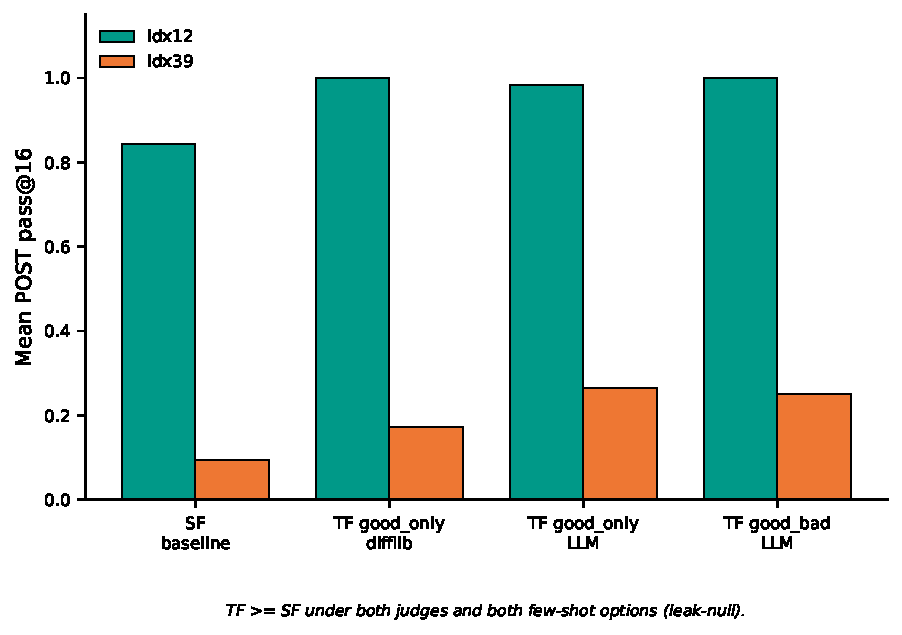
\includegraphics[width=0.85\linewidth]{../figures/fig_4_5_ablation.pdf}\end{center}

\textbf{Figure 4.5}
\emph{Judge × few-shot ablation, mean POST pass@16.} Teacher-first stays at or above the student-first baseline across both judges (difflib, LLM) and both few-shot options (good\_only, good\_bad); good\_bad ≈ good\_only indicates the leak is null on code.

\begin{center}\rule{0.5\linewidth}{0.5pt}\end{center}

\section{4.5 Math pilot: a boundary characterization}\label{math-pilot-a-boundary-characterization}

The math pilot extends the comparison to the domain where the advisor and Kim et al.~{[}2{]} expect leak and epistemic effects to be strongest. It is a pilot in the strict sense: 2 problems, a different model, and an answer-only reference (§3.5). It does not escape, and that non-escape is informative about \emph{when} teacher-first works.

\subsection{4.5.1 Setup and frontier scan}\label{setup-and-frontier-scan}

Gemma-4-E4B (thinking ON) on MathArena AIME 2026 {[}10{]} (30 problems, integer answers), \texttt{reference\_mode\ =\ ground\_truth} (the teacher always sees the correct answer, the extreme leak regime), LLM judge \texttt{glm-4.5-flash} with a derive-vs-copy prompt. A frontier scan (n\_samples = 2) spreads the problems out: frontier (0 \textless{} pass \textless{} 1) at idx 8, 11, 21, 25; too-hard (pass = 0) at 15 problems; ceiling (pass = 1) at 11 problems. Gemma-4 with thinking solves many AIME 2026 problems, so difficulty is scattered rather than monotone.

\begin{center}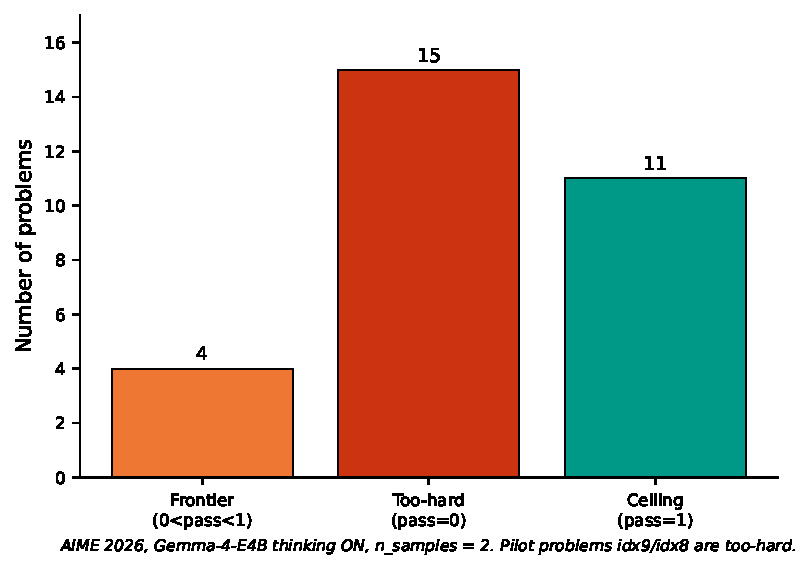
\includegraphics[width=0.85\linewidth]{../figures/fig_4_7_frontier_bands.pdf}\end{center}

\textbf{Figure 4.7}
\emph{AIME 2026 frontier-scan band membership.} Of 30 problems, 4 are frontier (0 \textless{} pass \textless{} 1), 15 too-hard (pass = 0), and 11 at ceiling (pass = 1). The two pilot problems (idx9, idx8) are drawn from the too-hard band.

\subsection{4.5.2 No escape on too-hard problems}\label{no-escape-on-too-hard-problems}

The first clean run, idx9 (triangle 13-14-15 rotated about the circumcenter, hexagon area, correct answer 156):

\begin{longtable}[]{@{}lll@{}}
\toprule\noalign{}
& PRE & POST \\
\midrule\noalign{}
\endhead
\bottomrule\noalign{}
\endlastfoot
pass\_rate & 0.000 & 0.000 \\
greedy & 0.000 & 0.000 \\
boxed answer & 148 & 168 \\
\end{longtable}

Discovery curve 1.00 → 1.00 → 1.00, with \texttt{n\_good=1,\ n\_bad=3} each step. Teacher-first does \textbf{not} pull the too-hard problem off zero. idx8 (a dice/sticker probability problem, correct answer 29) replicates this: labeled frontier by the noisy scan but actually PRE pass = 0 at 4 samples, PRE boxed 40201 → POST boxed 17, still wrong, PRE 0 → POST 0.

The reason is regime, not compute. With thinking ON and 16384 tokens (no truncation), the model reasons to completion and still answers wrong with confidence (148, 168). This rules out ``did not think enough'' and identifies a \textbf{capability ceiling}. Because the reference is only the number 156, the teacher can copy but has no in-reach method to distill, and distilling a few answer-aware traces cannot install a capability the model lacks. The code notion of ``hard'' is reachable-but-stuck (solvable once unblocked by feedback or best-in-batch); the AIME ``too-hard'' problems are beyond-capability. The wrong regime was selected, which is precisely the boundary the pilot characterizes.

\begin{center}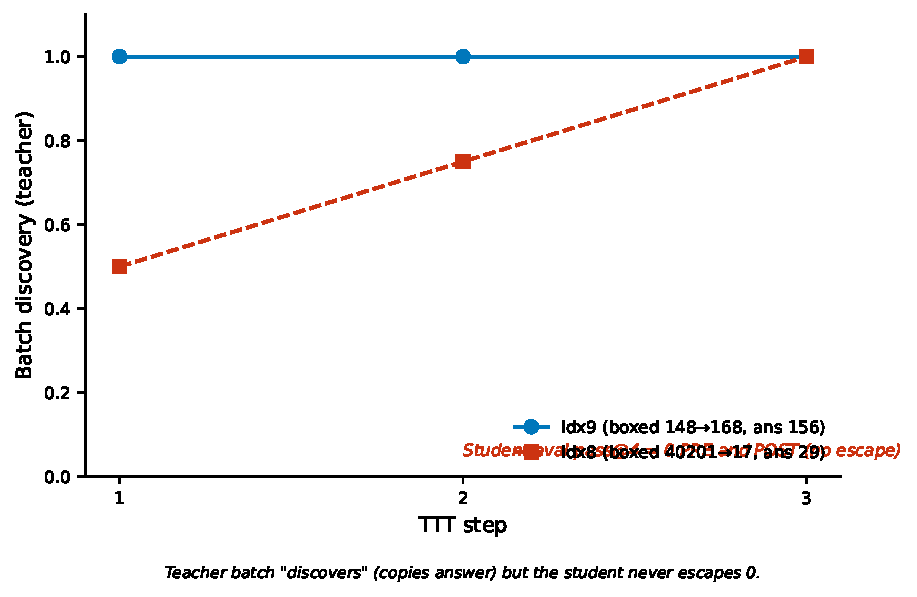
\includegraphics[width=0.85\linewidth]{../figures/fig_4_6_math_discovery.pdf}\end{center}

\textbf{Figure 4.6}
\emph{Math teacher-batch discovery versus student escape.} The teacher's batch ``discovers'' the answer across the three steps (it copies the leaked answer), yet the student's eval pass@4 stays at 0 both PRE and POST. The boxed answer drifts (148→168, 40201→17) without reaching the correct value, illustrating form changing while substance does not.

\subsection{4.5.3 Measured leak, and a fallback that defeats the judge}\label{measured-leak-and-a-fallback-that-defeats-the-judge}

Although the pilot does not escape, the judge measures the leak cleanly, which is an on-thesis positive. With the leaked answer 156, all four teacher trajectories are nominally ``correct'' every step (batch mean reward 1.0 across all three steps of idx9), yet the judge flags most of them as copies. Across the 12 judged trajectories (full verdict log in Appendix D):

\begin{longtable}[]{@{}
  >{\raggedright\arraybackslash}p{(\columnwidth - 4\tabcolsep) * \real{0.3333}}
  >{\raggedright\arraybackslash}p{(\columnwidth - 4\tabcolsep) * \real{0.3333}}
  >{\raggedright\arraybackslash}p{(\columnwidth - 4\tabcolsep) * \real{0.3333}}@{}}
\toprule\noalign{}
\begin{minipage}[b]{\linewidth}\raggedright
\end{minipage} & \begin{minipage}[b]{\linewidth}\raggedright
is\_copy = true (asserts 156)
\end{minipage} & \begin{minipage}[b]{\linewidth}\raggedright
genuine derivation (independent, rq ≥ 3)
\end{minipage} \\
\midrule\noalign{}
\endhead
\bottomrule\noalign{}
\endlastfoot
count (of 12) & \textbf{10 (≈83\%)} & \textbf{1} \\
\end{longtable}

The single genuine derivation appears only at step 1 (is\_copy=false, reasoning\_quality 4); at steps 2 and 3 every trajectory is a copy. The filter keeps one trajectory as good each step (\texttt{n\_good=1,\ n\_bad=3}), a 75\% per-step reject rate, but at steps 2--3 that one ``good'' is itself a copy retained by the keep-best-correct fallback (§3.3.3). So the privileged teacher mostly copies the answer rather than deriving it, the judge detects this, and this is measurable information leak, exactly the concern of {[}2{]} and the contrast with code, where leak is null (§4.4).

The idx8 log (run 463y4fjr) sharpens the second-order problem. There, \emph{every} judge verdict across all three steps is \texttt{is\_copy=true} (the single \texttt{is\_copy=false} has reasoning\_quality 2 \textless{} 3, so it is also bad). The \texttt{n\_good=1} per step therefore comes \emph{entirely} from the fallback: the good pool consists only of copies the judge already rejected. The fallback defeats the judge when the teacher produces nothing but copies. This is also a judge-degradation effect: the judge catches blatant copying but cannot reliably separate a genuine derivation from an answer-directed confabulation on beyond-capability problems, where both reach the right number.

\subsection{4.5.4 Epistemic pathology: form changes, substance does not}\label{epistemic-pathology-form-changes-substance-does-not}

Reading the full thinking traces shows what TTT actually transfers in the leak regime. The model satisfices toward a ``clean'' number: when stuck it assumes a value (PRE θ = 90°; POST Area = 2K = 168) and rationalizes it (``in problems of this nature, the intended answer is usually clean''), guessing by contest convention rather than deriving. It shows \textbf{epistemic suppression} {[}2{]}: it knows the problem is ambiguous (``this is impossible'', ``contradiction'') but does not admit it and emits a confident answer. It performs ``self-correction theater'', labeling steps ``Crucial Insight Check'' and ``Self-Correction'' while the correction loops without converging.

Most telling, POST is half the length (≈24k → 12k characters) with a better setup (it now knows cos C = 3/5, θ = 90° ± C) but gives up earlier and cuts a corner to a wrong answer (168). The student learns the teacher's \emph{confident reasoning style} from answer-aware traces but not its method. This is epistemic mimicry made visible: form transfers, substance does not. The model does not even memorize 156. idx8 runs the opposite direction (POST is \emph{more} rigorous, with casework) yet is still wrong, so TTT changes reasoning style in both directions without fixing correctness.

\subsection{4.5.5 Pilot conclusion}\label{pilot-conclusion}

Across two too-hard AIME problems, teacher-first does not escape, and the non-escape is consistent and interpretable: the teacher copies the answer (the judge catches roughly 75\%), the leak transfers form rather than substance (replicated across both problems), and the student stays at zero. Stated as a boundary: \textbf{teacher-first escapes when the reference provides an in-reach method (code, §4.2), and fails when the teacher has only the answer on a beyond-capability problem (AIME too-hard).} Escape requires reachable capability, not merely a correct answer. This contrast is stronger evidence about the mechanism than a ``works everywhere'' result would be.

\begin{center}\rule{0.5\linewidth}{0.5pt}\end{center}

\section{In-chapter citations}\label{in-chapter-citations}

Numbered per the master bibliography (\texttt{00\_references.md}): {[}1{]} Hübotter et al.~2026 · {[}2{]} Kim et al.~2026 · {[}7{]} Qwen3 · {[}10{]} MathArena AIME 2026. (Full method and metric definitions in Chapter 3.)

\input{_ch5.tex}
\input{_ch6.tex}
\input{_ch7.tex}

\renewcommand{\bibname}{References}
\begin{thebibliography}{99}
\addcontentsline{toc}{chapter}{References}

\bibitem{r1} J. Hübotter, F. Lübeck, L. Behric, A. Baumann, M. Bagatella, D. Marta, I. Hakimi, I. Shenfeld, T. Kleine Buening, C. Guestrin, A. Krause, ``Reinforcement Learning via Self-Distillation,'' arXiv:2601.20802, 2026. Code: \url{https://github.com/lasgroup/SDPO}.

\bibitem{r2} Kim et al., ``Why Self-Distillation Degrades: Suppression of Epistemic Verbalization from Rich Context,'' arXiv:2603.24472, 2026.

\bibitem{r3} I. Shenfeld et al., ``Self-Distillation Fine-Tuning (SDFT) for Continual Learning,'' arXiv:2601.19897, 2026.

\bibitem{r4} lasgroup, ``SDPO official codebase (verl fork),'' 2026. \url{https://github.com/lasgroup/SDPO}. (Scientific reference; KL config $\alpha=1.0$, top-$K=20$ for LCBv6.)

\bibitem{r5} HuggingFace, ``TRL v1.4.0 --- SDPO/SDFT Trainer documentation,'' 2026.

\bibitem{r6} N. Jain, K. Han, A. Gu, W.-D. Li, F. Yan, T. Zhang, S. Wang, A. Solar-Lezama, K. Sen, and I. Stoica, ``LiveCodeBench: Holistic and Contamination-Free Evaluation of Large Language Models for Code,'' arXiv:2403.07974, 2024.

\bibitem{r7} Qwen Team, ``Qwen3 Technical Report,'' arXiv:2505.09388, 2025.

\bibitem{r8} Z. Shao et al., ``DeepSeekMath: Pushing the Limits of Mathematical Reasoning in Open Language Models,'' arXiv:2402.03300, 2024. (Introduces GRPO.)

\bibitem{r9} M. Chen et al., ``Evaluating Large Language Models Trained on Code,'' arXiv:2107.03374, 2021. (pass@$k$.)

\bibitem{r10} MathArena, ``AIME 2026,'' HuggingFace dataset \texttt{MathArena/aime\_2026}, 2026. \url{https://huggingface.co/datasets/MathArena/aime_2026}.

\bibitem{r11} R. Agarwal et al., ``On-Policy Distillation of Language Models: Learning from Self-Generated Mistakes,'' arXiv:2306.13649, 2023. (GKD; generalized JSD, cited by Hübotter for JSD stability.)

\bibitem{r12} E. D. Dolan and J. J. Moré, ``Benchmarking optimization software with performance profiles,'' \emph{Math.\ Program.}, vol.~91, no.~2, pp.~201--213, 2002. (Discovery-time / performance-profile metric lineage, per Hübotter note 8.)

\bibitem{r13} G. Hinton, O. Vinyals, and J. Dean, ``Distilling the Knowledge in a Neural Network,'' arXiv:1503.02531, 2015. (Knowledge-distillation lineage anchor.)

\bibitem{r14} J. Schulman, F. Wolski, P. Dhariwal, A. Radford, and O. Klimov, ``Proximal Policy Optimization Algorithms,'' arXiv:1707.06347, 2017.

\bibitem{r15} L. Ouyang, J. Wu, X. Jiang, D. Almeida, C. L. Wainwright, P. Mishkin, C. Zhang, S. Agarwal, K. Slama, A. Ray, J. Schulman, J. Hilton, F. Kelton, L. Miller, M. Simens, A. Askell, P. Welinder, P. Christiano, J. Leike, and R. Lowe, ``Training Language Models to Follow Instructions with Human Feedback,'' arXiv:2203.02155, 2022. (InstructGPT / RLHF.)

\bibitem{r16} R. Rafailov, A. Sharma, E. Mitchell, S. Ermon, C. D. Manning, and C. Finn, ``Direct Preference Optimization: Your Language Model is Secretly a Reward Model,'' arXiv:2305.18290, 2023.

\bibitem{r17} J. Wei, X. Wang, D. Schuurmans, M. Bosma, B. Ichter, F. Xia, E. Chi, Q. Le, and D. Zhou, ``Chain-of-Thought Prompting Elicits Reasoning in Large Language Models,'' arXiv:2201.11903, 2022.

\bibitem{r18} X. Wang, J. Wei, D. Schuurmans, Q. Le, E. Chi, S. Narang, A. Chowdhery, and D. Zhou, ``Self-Consistency Improves Chain of Thought Reasoning in Language Models,'' arXiv:2203.11171, 2022.

\bibitem{r19} E. Zelikman, Y. Wu, J. Mu, and N. D. Goodman, ``STaR: Bootstrapping Reasoning With Reasoning,'' arXiv:2203.14465, 2022.

\bibitem{r20} B. Brown, J. Juravsky, R. Ehrlich, R. Clark, Q. V. Le, C. Ré, and A. Mirhoseini, ``Large Language Monkeys: Scaling Inference Compute with Repeated Sampling,'' arXiv:2407.21787, 2024.

\bibitem{r21} N. Muennighoff, Z. Yang, W. Shi, X. L. Li, L. Fei-Fei, H. Hajishirzi, L. Zettlemoyer, P. Liang, E. Cand\`es, and T. Hashimoto, ``s1: Simple Test-Time Scaling,'' arXiv:2501.19393, 2025.

\bibitem{r22} H. Lightman, V. Kosaraju, Y. Burda, H. Edwards, B. Baker, T. Lee, J. Leike, J. Schulman, I. Sutskever, and K. Cobbe, ``Let's Verify Step by Step,'' arXiv:2305.20050, 2023. (Process supervision.)

\bibitem{r23} S. Kadavath, T. Conerly, A. Askell, et al., ``Language Models (Mostly) Know What They Know,'' arXiv:2207.05221, 2022.

\bibitem{r24} Y. Kim and A. M. Rush, ``Sequence-Level Knowledge Distillation,'' in \emph{Proc. EMNLP}, arXiv:1606.07947, 2016.

\end{thebibliography}


\appendix
\chapter{Appendices}\label{appendices}

Appendices A--F are complete. B and C are reproduced verbatim from the codebase (\passthrough{\lstinline!07\_discovery\_curve.py!}, \passthrough{\lstinline!09\_teacher\_first.py!}); D from the W\&B \passthrough{\lstinline!output.log!} files (math pilot and a code exemplar); E/F from the W\&B export and reconciliation. The one remaining optional addition is the full idx0--90 code frontier-scan table (F.2), for which only the four problems actually used are listed.

\begin{center}\rule{0.5\linewidth}{0.5pt}\end{center}

\section{Appendix A --- Hyperparameters}\label{appendix-a-hyperparameters}

\subsection{A.1 Code (LiveCodeBench v6, core)}\label{a.1-code-livecodebench-v6-core}

\begin{longtable}[]{@{}ll@{}}
\toprule\noalign{}
Setting & Value \\
\midrule\noalign{}
\endhead
\bottomrule\noalign{}
\endlastfoot
Model & Qwen3-4B, LoRA r=32, bf16, thinking OFF \\
Optimizer & AdamW, lr = 1e-5 \\
TTT steps \(K\) & 15 \\
Teacher samples \passthrough{\lstinline!teacher\_n!} (TF) & 10 \\
\passthrough{\lstinline!num\_generations!} (SF baseline) & 4 \\
Teacher temperature & \textasciitilde1.0 \\
Eval samples \(N_{\text{eval}}\) & 16 (student-only, PRE and POST) \\
Seeds & 0, 1, 2, 3 (matched PRE per seed) \\
Template & T2 (anchor) for the main comparison; T1/T2/T5 for RQ1 \\
KL top-K & 20 \\
KL direction \(\alpha\) & 1.0 (reverse KL) \\
Importance-sampling clip & 2.0 \\
Similarity threshold (difflib judge) & \textasciitilde0.9 \\
Few-shot exemplars \passthrough{\lstinline!max\_fewshot!} & 3 \\
Few-shot option & good\_only (main); good\_bad (leak ablation) \\
Judge & difflib (string-sim) or groq \passthrough{\lstinline!llama-3.3-70b!} (semantic) \\
\passthrough{\lstinline!reference\_mode!} & best\_in\_batch \\
Hardware & Colab L4 (22 GB) / A100 \\
\end{longtable}

\subsection{A.2 Math (AIME 2026, pilot)}\label{a.2-math-aime-2026-pilot}

\begin{longtable}[]{@{}
  >{\raggedright\arraybackslash}p{(\columnwidth - 2\tabcolsep) * \real{0.5000}}
  >{\raggedright\arraybackslash}p{(\columnwidth - 2\tabcolsep) * \real{0.5000}}@{}}
\toprule\noalign{}
\begin{minipage}[b]{\linewidth}\raggedright
Setting
\end{minipage} & \begin{minipage}[b]{\linewidth}\raggedright
Value
\end{minipage} \\
\midrule\noalign{}
\endhead
\bottomrule\noalign{}
\endlastfoot
Model & google/gemma-4-E4B-it, LoRA all-linear, thinking ON \\
TTT steps \(K\) & 3 \\
Teacher samples \passthrough{\lstinline!teacher\_n!} & 4 \\
Eval samples & 4 \\
\passthrough{\lstinline!max\_new\_tokens!} & 16384 (8192 truncated \passthrough{\lstinline!\\boxed!}, producing spurious zeros) \\
Sampling & top\_p 0.95, top\_k 64 \\
\passthrough{\lstinline!reference\_mode!} & ground\_truth (leak regime) \\
Judge & \passthrough{\lstinline!zai:glm-4.5-flash!}, derive-vs-copy (\passthrough{\lstinline!is\_copy!} + \passthrough{\lstinline!reasoning\_quality!} 1--5) \\
Data & MathArena/aime\_2026 (30 problems, integer answers) \\
Hardware & Modal A100-80GB \\
\end{longtable}

Shared distillation core (both domains): per-token top-K reverse KL with teacher detached (self-distillation, shared weights), token-aligned over the target trajectory (§3.3.5).

\begin{center}\rule{0.5\linewidth}{0.5pt}\end{center}

\section{Appendix B --- Reprompt templates (verbatim)}\label{appendix-b-reprompt-templates-verbatim}

Each preset overrides the SDPO template \emph{slots} only; the model, the feedback content (the privileged context), and the hyperparameters are held fixed for a clean ablation. The TRL 1.6.0 slots are \passthrough{\lstinline!reprompt\_template → \{prompt\}\{solution\}\{feedback\}!}, \passthrough{\lstinline!feedback\_template → \{feedback\_raw\}!} (this \passthrough{\lstinline!\{feedback\_raw\}!} is the privileged context), and \passthrough{\lstinline!solution\_template → \{successful\_previous\_attempt\}!}. T2 is the TRL/paper default verbatim.

\textbf{Honest scope note.} The codebase (\passthrough{\lstinline!07\_discovery\_curve.py!}, \passthrough{\lstinline!REPROMPT\_TEMPLATES!}) implements \textbf{four} presets, reproduced below: T1, T2, T5, T6. The taxonomy of §3.4 also names T3 (verbose), T4 (structured JSON), and T7 (cumulative history); these three are conceptual points in the design space and were \textbf{not} implemented. Of the four implemented, the experiments probe T1/T2/T5 (§4.3); T6 is implemented but unprobed.

\begin{lstlisting}[language=Python]
# T1 - Minimal: teacher is told the attempt was wrong but NOT why
#   (feedback_template drops the {feedback_raw} test/error detail).
"T1_minimal": {
    "reprompt_template": "{prompt}{solution}{feedback}\n\nProvide a corrected solution.\n",
    "feedback_template": "\nYour previous attempt was incorrect.\n\n",
},
# T2 - Standard / anchor: exact TRL + paper defaults (rich feedback included).
"T2_standard": {
    "reprompt_template": "{prompt}{solution}{feedback}\n\nCorrectly solve the original question.\n",
    "feedback_template": "\nThe following is feedback from your unsuccessful earlier attempt:\n\n{feedback_raw}\n\n",
},
# T5 - Reasoning-inducing: SAME rich feedback as T2, trailing instruction asks
#   for root-cause analysis first.
"T5_reasoning": {
    "reprompt_template": "{prompt}{solution}{feedback}\n\nFirst, identify the root cause of the failure, then provide a corrected solution.\n",
    "feedback_template": "\nThe following is feedback from your unsuccessful earlier attempt:\n\n{feedback_raw}\n\n",
},
# T6 - First-person: SAME rich feedback, reframed as the model's own reflection.
"T6_first_person": {
    "reprompt_template": "{prompt}{solution}{feedback}\n\nI attempted this problem and my solution was incorrect. Let me reconsider and write a correct solution.\n",
    "feedback_template": "\nHere is the feedback from my unsuccessful earlier attempt:\n\n{feedback_raw}\n\n",
},
\end{lstlisting}

\begin{center}\rule{0.5\linewidth}{0.5pt}\end{center}

\section{Appendix C --- Teacher and judge prompts (verbatim)}\label{appendix-c-teacher-and-judge-prompts-verbatim}

\subsection{C.1 Teacher prompt and few-shot block}\label{c.1-teacher-prompt-and-few-shot-block}

The teacher prompt is \passthrough{\lstinline!question + few-shot block + feedback + trailing instruction!}, where the feedback and trailing instruction come from the selected reprompt preset (Appendix B). A worked instance of the assembled prompt (with the leaked math reference) is shown in Appendix D.1. The few-shot block (\passthrough{\lstinline!09\_teacher\_first.py!}, \passthrough{\lstinline!\_build\_fewshot\_block!}) is assembled as follows; exemplars are stripped of their thinking traces and capped at 1500 characters:

\begin{lstlisting}
Here are correct, independent example solutions:

Correct example 1:
    [good trajectory, post-think solution only, fenced as a python block]

[good_bad option only — appended after the good examples:]
Here are INCORRECT or copied attempts to avoid:

Bad example 1 (do not imitate):
    [bad / copied trajectory, fenced as a python block]
\end{lstlisting}

Under \passthrough{\lstinline!good\_only!} (Option 2) only the ``Correct example'' exemplars appear; under \passthrough{\lstinline!good\_bad!} (Option 1) the ``Bad example'' block is appended, which is what re-introduces reference-like content (§3.3.4).

\subsection{\texorpdfstring{C.2 LLM judge prompt --- code (groq \texttt{llama-3.3-70b})}{C.2 LLM judge prompt --- code (groq llama-3.3-70b)}}\label{c.2-llm-judge-prompt-code-groq-llama-3.3-70b}

\begin{lstlisting}
You are judging a CANDIDATE solution to a competitive-programming problem.

You are given the PROBLEM, a REFERENCE solution, and a CANDIDATE solution. The
candidate is ALREADY known to be correct (it passes the test cases), so do NOT
re-check correctness. Decide only two things:

  1. is_copy: Is the candidate essentially a copy of the reference solution --
     i.e. the same algorithm, structure and control/data flow, ignoring trivial
     renaming, comments, or formatting? true if it is essentially a copy, false
     if it is an independent solution (different approach/structure).
  2. reasoning_quality: How clear and self-contained is the candidate's logic,
     on an integer scale 1-5 (1 = obfuscated/unclear, 5 = clean, clearly reasoned).

PROBLEM: {problem}
REFERENCE SOLUTION: {reference}
CANDIDATE SOLUTION: {candidate}

Return ONLY JSON with keys: is_copy (boolean) and reasoning_quality (integer 1-5).
\end{lstlisting}

\subsection{\texorpdfstring{C.3 LLM judge prompt --- math (\texttt{glm-4.5-flash})}{C.3 LLM judge prompt --- math (glm-4.5-flash)}}\label{c.3-llm-judge-prompt-math-glm-4.5-flash}

\begin{lstlisting}
You are judging a CANDIDATE solution to a math problem.

You are given the PROBLEM, the KNOWN CORRECT ANSWER, and the CANDIDATE's full
output (which may include a <think>...</think> reasoning block followed by a final
\boxed{answer}). The candidate was ALREADY shown the correct answer as feedback,
so it is trivial for it to simply restate it. Decide only two things:

  1. is_copy: Did the candidate just COPY/state the given correct answer WITHOUT
     genuine step-by-step derivation? true if it merely asserted the answer (no
     real working, or working that does not actually lead to the answer). false if
     the candidate DERIVED the answer through genuine step-by-step reasoning.
  2. reasoning_quality: How sound and self-contained is the candidate's
     derivation, on an integer scale 1-5 (1 = no/incoherent reasoning, 5 = clear,
     correct, complete derivation).

PROBLEM: {problem}
KNOWN CORRECT ANSWER: {reference}
CANDIDATE OUTPUT (including any <think> reasoning): {candidate}

Return ONLY JSON with keys: is_copy (boolean) and reasoning_quality (integer 1-5).
\end{lstlisting}

The judge returns structured JSON (\passthrough{\lstinline!is\_copy!}: boolean, \passthrough{\lstinline!reasoning\_quality!}: integer). Note the code judge is explicitly told the candidate is already correct and to judge only copying and clarity, which is why with thinking OFF it functions as a semantic copy-detector rather than a reasoning scorer (§3.3.3).

\begin{center}\rule{0.5\linewidth}{0.5pt}\end{center}

\section{Appendix D --- Example trajectories (math pilot)}\label{appendix-d-example-trajectories-math-pilot}

Excerpts are verbatim from the W\&B \passthrough{\lstinline!output.log!} of each run; long completions are trimmed with \passthrough{\lstinline![...]!}. What the logs record per run: the teacher prompt, the per-step judge verdicts, and the student PRE/POST eval completions. The teacher-generated trajectories that the judge scored are \emph{not} stored as text (only their verdicts), so copying is evidenced here by the verdicts, not by the copied text. The math excerpts (D.1--D.4) show the form-not-substance failure; the code excerpt (D.5) shows the contrasting genuine discovery.

\subsection{\texorpdfstring{D.1 Teacher prompt with the leaked reference (idx9, run \texttt{fi5m0as1})}{D.1 Teacher prompt with the leaked reference (idx9, run fi5m0as1)}}\label{d.1-teacher-prompt-with-the-leaked-reference-idx9-run-fi5m0as1}

\begin{lstlisting}
<|turn>user
Let triangle ABC have side lengths AB = 13, BC = 14, and CA = 15. Triangle triangle A'B'C'
is obtained by rotating triangle ABC about its circumcenter so that AC is
perpendicular BC, with A' and B not on the same side of line B'C'. Find the
integer closest to the area of hexagon AA'CC'BB'.

The following is feedback from your unsuccessful earlier attempt:

Reference: the correct final answer is 156.

Correctly solve the original question.
[...]
\end{lstlisting}

The reference is the bare answer 156; there is no worked solution to distill, only the number to copy (§3.5).

\subsection{D.2 Judge verdict sequences}\label{d.2-judge-verdict-sequences}

idx9 (run \passthrough{\lstinline!fi5m0as1!}), correct answer 156; batch reward 1.0 every step, so all 12 trajectories are nominally correct:

\begin{longtable}[]{@{}lll@{}}
\toprule\noalign{}
step & verdicts (is\_copy / reasoning\_quality) & n\_good / n\_bad \\
\midrule\noalign{}
\endhead
\bottomrule\noalign{}
\endlastfoot
1 & (T,1) (T,2) (F,2) (F,4) & 1 / 3 \\
2 & (T,2) (T,2) (T,2) (T,3) & 1 / 3 \\
3 & (T,2) (T,2) (T,1) (T,3) & 1 / 3 \\
\end{longtable}

The only genuine derivation (F,4) is at step 1; steps 2--3 are all copies, so the kept ``good'' comes from the fallback. idx8 (run \passthrough{\lstinline!463y4fjr!}), correct answer 29:

\begin{longtable}[]{@{}llll@{}}
\toprule\noalign{}
step & verdicts & n\_good / n\_bad & batch reward \\
\midrule\noalign{}
\endhead
\bottomrule\noalign{}
\endlastfoot
1 & (T,1) (T,3) & 1 / 1 & 0.50 \\
2 & (T,3) (T,2) (T,1) & 1 / 2 & 0.75 \\
3 & (T,4) (T,3) (T,2) (F,2) & 1 / 3 & 1.00 \\
\end{longtable}

Every idx8 verdict is \passthrough{\lstinline!is\_copy=true!} (the lone \passthrough{\lstinline!F!} has reasoning\_quality 2 \textless{} 3), so every kept ``good'' is a fallback-retained copy.

\subsection{D.3 Form changes, substance does not (idx9 student eval, PRE vs POST)}\label{d.3-form-changes-substance-does-not-idx9-student-eval-pre-vs-post}

\textbf{PRE} (23,920 chars, boxed \textbf{148}). The model recognizes the configuration is contradictory, then satisfices toward a clean angle:

\begin{quote}
``But \(AC \perp BC\) is impossible in \(\triangle ABC\) {[}\ldots{]} \textbf{Crucial Insight Check:} {[}\ldots{]} This seems overly complex for a calculation intended to yield a clean integer answer nearby. Let's pivot and assume \(\theta\) is a `nice' angle, like \(90^\circ\) or \(180^\circ\) {[}\ldots{]}''
\end{quote}

It computes 315.5 under one reading, reinterprets the hexagon as a union (147.5), and boxes 148.

\textbf{POST} (11,951 chars, about half the length, boxed \textbf{168}). After TTT the setup is better --- it now derives \(\cos C = 3/5\) and \(\theta = 90^\circ \pm C\) --- but it gives up earlier and shortcuts to twice the triangle area:

\begin{quote}
``{[}\ldots{]} unless the overlap is significant {[}\ldots{]} the area is often closely approximated by the sum of the individual areas {[}\ldots{]} the most straightforward interpretation leading to a clean integer answer is that the intended area calculation ignores the slight overlap {[}\ldots{]} \(\text{Area}(H) \approx 84 + 84 = 168\).''
\end{quote}

Both are wrong (correct 156); the model never reaches or memorizes the leaked answer. TTT changed the reasoning style (more confident, more willing to shortcut), not the capability.

\subsection{D.4 The opposite stylistic drift (idx8 student eval, PRE vs POST)}\label{d.4-the-opposite-stylistic-drift-idx8-student-eval-pre-vs-post}

idx8 drifts the other way. \textbf{PRE} (boxed \textbf{40201}) treats the rolls as independent and computes \(p = 2^{13}\cdot 3 / 5^6\), giving \(m+n = 24576 + 15625 = 40201\). \textbf{POST} (boxed \textbf{17}) is \emph{more} rigorous --- it does casework on \(R_2 = R_4\) versus \(R_2 \neq R_4\), counts \(N_B = 11700\) and \(N_{A\cap B} = 3600\), and simplifies \(p = 4/13\) to \(m+n = 17\). POST is longer and more careful, yet still wrong (correct 29). Across the two problems, then, TTT moves the reasoning style in opposite directions (idx9 lazier, idx8 more rigorous) while leaving correctness unchanged.

\subsection{\texorpdfstring{D.5 Genuine discovery on code (idx12, run \texttt{teacherfirst-...-idx12})}{D.5 Genuine discovery on code (idx12, run teacherfirst-...-idx12)}}\label{d.5-genuine-discovery-on-code-idx12-run-teacherfirst-...-idx12}

The contrast with the math pilot is the point of the thesis. Here the output is a \emph{program}, and teacher-first installs a working one. Problem \passthrough{\lstinline!abc389\_b!}: given \(X\), find \(N\) with \(N! = X\).

\textbf{PRE} (greedy score 0.075, pass@16 = 0.000). The student inverts the task, computing a factorial instead of finding \(N\), which also overflows the integer-string limit on large inputs:

\begin{lstlisting}[language=Python]
import math
X = int(input())
print(math.factorial(X))
\end{lstlisting}

\textbf{Execution feedback} (the privileged context --- this is what ``execution-guided'' means):

\begin{lstlisting}
Your solution must satisfy these test cases:
- Input: 6  ->  Expected: 3
- Input: 2432902008176640000  ->  Expected: 20
Result of running your earlier attempt:
Runtime Error
ValueError: Exceeds the limit (4300 digits) for integer string conversion ...
Last Executed Input: 5040
\end{lstlisting}

\textbf{POST} (greedy score 1.000, pass@16 = 1.000). The student now iterates to find \(N\), a correct algorithm that generalizes to any input:

\begin{lstlisting}[language=Python]
import sys
def find_n_factorial(X):
    n = 1
    current = 1
    while current < X:
        n += 1
        current *= n
    return n
def main():
    X = int(sys.stdin.readline())
    print(find_n_factorial(X))
if __name__ == "__main__":
    main()
\end{lstlisting}

PRE pass 0.000 → POST pass 1.000 (discovery curve 0.85 → 1.0 → \ldots{} → 1.0; greedy 0.075 → 1.0). Unlike the math pilot, the distilled output is a method: a program that solves the problem for every input, not a value to copy. This is the value-versus-procedure boundary (Chapter 5) made concrete.

\begin{center}\rule{0.5\linewidth}{0.5pt}\end{center}

\section{Appendix E --- Per-seed results}\label{appendix-e-per-seed-results}

\subsection{E.1 idx39 (abc393\_d, hard, base pass ≈ 0.1), eval-16, difflib judge}\label{e.1-idx39-abc393_d-hard-base-pass-0.1-eval-16-difflib-judge}

\begin{longtable}[]{@{}llll@{}}
\toprule\noalign{}
seed & PRE & TF POST & SF POST \\
\midrule\noalign{}
\endhead
\bottomrule\noalign{}
\endlastfoot
0 & 0.000 & 0.438 & 0.188 \\
1 & 0.000 & 0.062 & 0.000 \\
2 & 0.062 & 0.125 & 0.125 \\
3 & 0.188 & 0.062 & 0.062 \\
mean & & 0.172 & 0.094 \\
\end{longtable}

\subsection{E.2 idx12 (abc389\_b, model-hard, model pass ≈ 0.12), eval-16}\label{e.2-idx12-abc389_b-model-hard-model-pass-0.12-eval-16}

\begin{longtable}[]{@{}llll@{}}
\toprule\noalign{}
seed & PRE & TF POST & SF POST \\
\midrule\noalign{}
\endhead
\bottomrule\noalign{}
\endlastfoot
0 & 0.000 & 1.000 & 0.938 \\
1 & 0.062 & 1.000 & 0.500 \\
2 & 0.062 & 1.000 & 1.000 \\
3 & 0.125 & 1.000 & 0.938 \\
mean & & 1.000 & 0.844 \\
\end{longtable}

\subsection{E.3 Hard-frontier means and escape-zero instances}\label{e.3-hard-frontier-means-and-escape-zero-instances}

\begin{longtable}[]{@{}
  >{\raggedright\arraybackslash}p{(\columnwidth - 12\tabcolsep) * \real{0.1429}}
  >{\raggedright\arraybackslash}p{(\columnwidth - 12\tabcolsep) * \real{0.1429}}
  >{\raggedright\arraybackslash}p{(\columnwidth - 12\tabcolsep) * \real{0.1429}}
  >{\raggedright\arraybackslash}p{(\columnwidth - 12\tabcolsep) * \real{0.1429}}
  >{\raggedright\arraybackslash}p{(\columnwidth - 12\tabcolsep) * \real{0.1429}}
  >{\raggedright\arraybackslash}p{(\columnwidth - 12\tabcolsep) * \real{0.1429}}
  >{\raggedright\arraybackslash}p{(\columnwidth - 12\tabcolsep) * \real{0.1429}}@{}}
\toprule\noalign{}
\begin{minipage}[b]{\linewidth}\raggedright
problem
\end{minipage} & \begin{minipage}[b]{\linewidth}\raggedright
id
\end{minipage} & \begin{minipage}[b]{\linewidth}\raggedright
judge
\end{minipage} & \begin{minipage}[b]{\linewidth}\raggedright
SF mean
\end{minipage} & \begin{minipage}[b]{\linewidth}\raggedright
TF mean
\end{minipage} & \begin{minipage}[b]{\linewidth}\raggedright
win/tie/loss
\end{minipage} & \begin{minipage}[b]{\linewidth}\raggedright
escape-zero seeds
\end{minipage} \\
\midrule\noalign{}
\endhead
\bottomrule\noalign{}
\endlastfoot
idx39 & abc393\_d & difflib & 0.094 & 0.172 & 2/2/0 & s1 (SF 0→0, TF 0.062) \\
idx64 & abc397\_e & LLM-groq & 0.047 & 0.422 & 4/0/0 & s1 (SF 0.062→0, TF 0.375), s2 (SF 0→0, TF 0.062) \\
idx77 & abc399\_f & difflib & 0.203 & 0.344 & 3/1/0 & --- \\
\end{longtable}

Per-seed POST pass@16 for idx64 and idx77, recovered from the W\&B export and reconciled to the published means (canonical runs: idx64 = LLM judge, idx77 = difflib, both good\_only / T2; dedup to the latest run per seed; \passthrough{\lstinline!data/reconcile.py!}):

\begin{longtable}[]{@{}lllll@{}}
\toprule\noalign{}
seed & idx64 TF & idx64 SF & idx77 TF & idx77 SF \\
\midrule\noalign{}
\endhead
\bottomrule\noalign{}
\endlastfoot
0 & 0.5625 & 0.000 & 0.250 & 0.0625 \\
1 & 0.375 & 0.0625 & 0.3125 & 0.250 \\
2 & 0.0625 & 0.000 & 0.6875 & 0.375 \\
3 & 0.625 & 0.125 & 0.125 & 0.125 \\
mean & 0.406 & 0.047 & 0.344 & 0.203 \\
\end{longtable}

\begin{quote}
The idx64 TF mean from these canonical runs is 0.406 versus the 0.422 reported in §4.2.3; the difference is which re-run is selected. Note also that the canonical idx64 seed-1 SF run here is 0.0625, whereas the escape-zero instance in §4.2.3 (SF → 0) is a different run of the same seed: the stuck-at-zero behavior is \textbf{run-dependent} (§6.1.1).
\end{quote}

\subsection{E.4 RQ1 template (SF arm, 2 seeds), POST pass@16}\label{e.4-rq1-template-sf-arm-2-seeds-post-pass16}

\begin{longtable}[]{@{}lll@{}}
\toprule\noalign{}
Template & idx12 (easy) & idx39 (hard) \\
\midrule\noalign{}
\endhead
\bottomrule\noalign{}
\endlastfoot
T1\_minimal & 0.66 & 0.03 \\
T2\_standard & 0.97 & 0.06 \\
T5\_reasoning & 0.97 & 0.13 \\
\end{longtable}

T5 on idx39 is stable across its two seeds (.125 / .125).

\subsection{E.5 Judge × few-shot ablation, mean POST pass (4 seeds)}\label{e.5-judge-few-shot-ablation-mean-post-pass-4-seeds}

\begin{longtable}[]{@{}lll@{}}
\toprule\noalign{}
arm & idx39 & idx12 \\
\midrule\noalign{}
\endhead
\bottomrule\noalign{}
\endlastfoot
SF baseline & 0.094 & 0.844 \\
TF · good\_only · difflib & 0.172 & 1.000 \\
TF · good\_only · LLM & 0.266 & 0.984 \\
TF · good\_bad · LLM & 0.250 & 1.000 \\
\end{longtable}

\begin{center}\rule{0.5\linewidth}{0.5pt}\end{center}

\section{Appendix F --- Frontier scans}\label{appendix-f-frontier-scans}

\subsection{F.1 Math (AIME 2026, Gemma-4-E4B thinking ON, n\_samples = 2)}\label{f.1-math-aime-2026-gemma-4-e4b-thinking-on-n_samples-2}

\begin{longtable}[]{@{}
  >{\raggedright\arraybackslash}p{(\columnwidth - 2\tabcolsep) * \real{0.5000}}
  >{\raggedright\arraybackslash}p{(\columnwidth - 2\tabcolsep) * \real{0.5000}}@{}}
\toprule\noalign{}
\begin{minipage}[b]{\linewidth}\raggedright
Band
\end{minipage} & \begin{minipage}[b]{\linewidth}\raggedright
Problem indices
\end{minipage} \\
\midrule\noalign{}
\endhead
\bottomrule\noalign{}
\endlastfoot
Frontier (0 \textless{} pass \textless{} 1) & 8, 11, 21, 25 \\
Too-hard (pass = 0) & 2, 3, 9, 10, 12, 13, 14, 16, 17, 22, 24, 26, 27, 28, 29 \\
Ceiling (pass = 1) & 0, 1, 4, 5, 6, 7, 15, 18, 19, 20, 23 \\
\end{longtable}

The two pilot problems (idx9, idx8) are drawn from the too-hard band; idx8 was labeled frontier by the noisy 2-sample scan but is actually pass = 0 at 4 samples.

\subsection{F.2 Code (LiveCodeBench v6, Qwen3-4B)}\label{f.2-code-livecodebench-v6-qwen3-4b}

Problems for the matched comparisons were selected by \emph{model} pass-rate \(\in (0,1)\) over a scan of idx0--90. The problems used are idx12 (abc389\_b), idx39 (abc393\_d), idx64 (abc397\_e), and idx77 (abc399\_f).

\begin{quote}
\textbf{To be completed:} the full idx0--90 model-pass-rate scan table is in the logs and should be reproduced here for completeness.
\end{quote}


\end{document}
